前一節中,通過假設程序中的循環最終都會結束,編譯器能夠優化某些循環和包含這些循環的代碼。優化器使用的基本邏輯是相同的:首先,假設程序不顯示UB。然後,推導出必須為真的條件,使這個假設成立,並假設這些條件確實總是為真。最後,在這種假設下有效的優化都可以進行。如果違反了假設,優化器生成的代碼會什麼,我們無法知道(除了已經提到的限制,仍是在同一臺計算機執行一些指令)。

標準中記錄的每一個UB案例都可以轉換為一個可優化的示例(特定的編譯器是否能利用這一點就是另一回事了)。我們再看幾個例子。

之前提到的,上溢有符號整數的結果是沒有定義。編譯器可以假設這種情況永遠不會發生,並且使用正數對有符號整數進行遞增,會得到一個更大的整數。編譯器真的會執行這種優化嗎?讓我們來找找答案。比較\texttt{f()}和\texttt{g()}這兩個函數:

\hspace*{\fill} \\ %插入空行
\noindent
\textbf{03\_int\_overflow.C}
\begin{lstlisting}[style=styleCXX]
bool f(int i) { return i + 1 > i; }
bool g(int i) { return true; }
\end{lstlisting}

定義良好的行為範圍內,這些函數是相同的。可以對它們進行基準測試,以確定編譯器是否會優化掉\texttt{f()}中的整個表達式。但如在前一章中看到的,有一種更可靠的方法。如果兩個函數生成相同的彙編碼,那麼它們肯定是相同的。 

%\hspace*{\fill} \\ %插入空行
\begin{center}
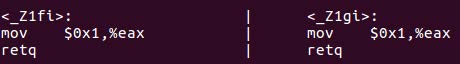
\includegraphics[width=0.7\textwidth]{content/3/chapter11/images/1.jpg}\\
圖11.1 - GCC9生成的\texttt{f()}(左)和\texttt{g()}(右)函數的x86彙編輸出
\end{center}

圖11.1中,打開優化後,GCC確實為兩個函數生成了相同的代碼(Clang也是如此)。彙編中出現的函數的名稱是所謂的“錯誤名稱”:因為C++允許有不同參數列表的函數具有相同的名稱,所以編譯器必須為每個這樣的函數生成一個唯一的名稱,通過將所有參數的類型編碼到對象代碼中實際使用的名稱中來進行實現。

如果想驗證這段代碼確實沒有\texttt{?:}操作符的痕跡,最簡單的方法是將\texttt{f()}函數與使用無符號整數進行相同計算的函數進行比較。參考以下代碼:

\hspace*{\fill} \\ %插入空行
\noindent
\textbf{03\_int\_overflow.C}
\begin{lstlisting}[style=styleCXX]
bool f(int i) { return i + 1 > i; }
bool h(unsigned int i) { return i + 1 > i; }
\end{lstlisting}

無符號整數的溢出有良好的定義,\texttt{i + 1}是大於\texttt{i}不總是正確。

%\hspace*{\fill} \\ %插入空行
\begin{center}
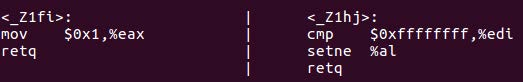
\includegraphics[width=0.9\textwidth]{content/3/chapter11/images/2.jpg}\\
圖11.2 - GCC9生成的\texttt{f()}(左)和\texttt{h()}(右)函數的x86彙編輸出
\end{center}

\texttt{h()}函數產生不同的代碼,cmp指令會進行比較,不熟悉x86彙編也可以猜到。在左邊,\texttt{f()}將載入常量0x1(布爾值也稱為true),並將結果放在寄存器EAX中用於返回。 

這個例子還演示了試圖推理UB或將其視為實現定義的危險。若程序將對整數做某種加法,當它溢出,特定的硬件將執行相應的操作,那麼將得到錯誤的結果。編譯器(有些編譯器確實如此)生成的代碼可能根本不需要遞增指令。

現在,有了足夠的知識來充分說明第2章中埋下的問題。在那一章中,我們觀察到同一個函數的兩個幾乎相同的實現之間的性能差異。該函數的工作是一個字符一個字符地比較兩個字符串,如果第一個字符串的字典序比第一個字符串大,則返回true。這是最簡實現:

\hspace*{\fill} \\ %插入空行
\noindent
\textbf{04a\_compare1.C}
\begin{lstlisting}[style=styleCXX]
bool compare1(const char* s1, const char* s2) {
	if (s1 == s2) return false;
	for (unsigned int i1 = 0, i2 = 0;; ++i1, ++i2) {
		if (s1[i1] != s2[i2]) return s1[i1] > s2[i2];
	}
}
\end{lstlisting}

這個函數用於對字符串進行排序,因此基準測試測量了對特定輸入字符串集進行排序的時間:

%\hspace*{\fill} \\ %插入空行
\begin{center}
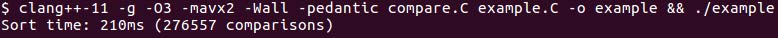
\includegraphics[width=0.9\textwidth]{content/3/chapter11/images/3.jpg}\\
圖11.3 -使用\texttt{compare1()}函數進行字符串比較的排序基準測試
\end{center}

比較實現非常簡單,這段代碼中沒有什麼不必要的東西。然而,令人驚訝的結果是,這是代碼性能最差的版本之一。表現最好的版本幾乎是一樣的:

\hspace*{\fill} \\ %插入空行
\noindent
\textbf{04b\_compare2.C}
\begin{lstlisting}[style=styleCXX]
bool compare2(const char* s1, const char* s2) {
	if (s1 == s2) return false;
	for (int i1 = 0, i2 = 0;; ++i1, ++i2) {
		if (s1[i1] != s2[i2]) return s1[i1] > s2[i2];
	}
}
\end{lstlisting}

唯一的區別是循環變量的類型:\texttt{unsigned int (compare1())}和\texttt{int (compare2())}。但索引不是負的,這應該沒有任何區別,但實際的性能差異很大:

%\hspace*{\fill} \\ %插入空行
\begin{center}
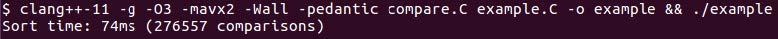
\includegraphics[width=0.9\textwidth]{content/3/chapter11/images/4.jpg}\\
圖11.4 - 使用\texttt{compare2()}函數進行字符串比較的排序基準測試
\end{center}

這種顯著的性能差異的原因與UB有關。為了理解發生了什麼,必須再次檢查彙編碼。圖11.5顯示了GCC為這兩個函數生成的代碼(只顯示了最相關的部分,字符串比較循環):

%\hspace*{\fill} \\ %插入空行
\begin{center}
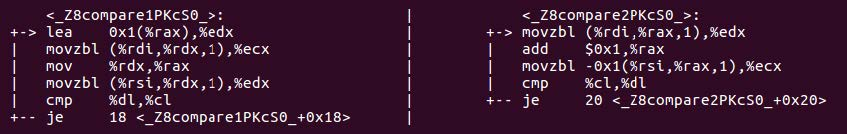
\includegraphics[width=0.9\textwidth]{content/3/chapter11/images/5.jpg}\\
圖11.5 - 為\texttt{compare1()}(左)和\texttt{compare2()}(右)函數生成的x86彙編碼
\end{center}

代碼看起來非常相似,只有一個不同。在右邊(\texttt{compare2()})中,可以看到add指令,它用於將循環索引加1(編譯器通過用一個循環變量替換兩個循環變量來優化代碼)。在左邊,沒有看起來像加法或增量的指令。取而代之的是lea指令,它表示加載和擴展地址,這裡用這種方式將索引變量增加1(進行了同樣的優化,只有一個循環變量)。 

現在,應該能夠猜到為什麼編譯器必須生成不同的代碼。雖然開發者期望索引永遠不會溢出,但是編譯器不能做這樣的假設。注意,兩個版本都使用32位整數,但是代碼是為64位機器生成的。如果一個32位的帶符號int溢出,結果是未定義的,所以在這種情況下,編譯器會假設溢出永遠不會發生。如果操作沒有溢出,則加法指令產生正確的結果。對於\texttt{unsigned int},編譯器必須考慮溢出的可能性,遞增\texttt{UINT\_MAX}應該得到0。但事實證明,x86-64上的add指令沒有這些語義。相反,它將結果擴展為一個64位整數。x86上32位無符號整數算法的最佳選擇是lea指令,它可以完成這項工作,但速度要慢得多。

這個示例演示瞭如何從程序定義良好且UB從未發生的假設往回推,編譯器可以啟用非常有效的優化,最終使整個排序操作快幾倍。

既然已經理解了代碼中發生的事情,就可以解釋代碼的其他幾個版本的行為了。首先,使用64位整數,有符號的或無符號的,提供與32位有符號整數相同的性能,編譯器將使用add(對於64位的無符號值,確實有正確的溢出語義)。其次,如果使用了最大索引,或者字符串長度,編譯器將推斷出索引不會溢出:

\begin{lstlisting}[style=styleCXX]
bool compare1(const char* s1, const char* s2,
unsigned int len) {
	if (s1 == s2) return false;
	for (unsigned int i1 = 0, i2 = 0; i1 < len; ++i1, ++i2) {
		if (s1[i1] != s2[i2]) return s1[i1] > s2[i2];
	}
	return false;
}
\end{lstlisting}

不必要的長度比較使得這個版本比最好的版本稍微慢一些。要避免意外地遇到這個問題,最可靠的方法是始終使用有符號循環變量或硬件本地大小的無符號整數(因此,除非真的需要,否則避免在64位處理器上執行無符號整型運算)。

可以使用標準中描述為未定義行為的其他情況,構造類似的演示(儘管不能保證特定的編譯器會利用可能的優化)。下面是使用指針解引用的例子:

\hspace*{\fill} \\ %插入空行
\noindent
\textbf{06a\_null.C}
\begin{lstlisting}[style=styleCXX]
int f(int* p) {
	++(*p);
	return p ? *p : 0; // Optimized to: return *p
}
\end{lstlisting}

這是一種常見的情況的簡化,開發者編寫了指針檢查代碼,以防止空指針,但並沒有在所有地方這樣做。如果輸入參數是空指針,則第二行(增量)是UB,這意味著整個程序的行為未定義,因此編譯器可以假設它從未發生。對彙編代碼的檢查表明,第三行中的比較被消除了:

%\hspace*{\fill} \\ %插入空行
\begin{center}
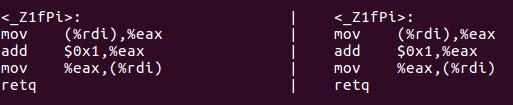
\includegraphics[width=0.9\textwidth]{content/3/chapter11/images/6.jpg}\\
圖11.6 -帶(左)和不帶(右)操作符的\texttt{f()}函數生成的x86彙編碼
\end{center}

如果先做指針檢查,也會發生同樣的情況:

\hspace*{\fill} \\ %插入空行
\noindent
\textbf{07a\_null.C}
\begin{lstlisting}[style=styleCXX]
int f(int* p) {
	if (p) ++(*p);
	return *p;
}
\end{lstlisting}

同樣,對彙編代碼的檢查表明,指針比較已經消除了,儘管到目前為止的程序行為都定義得很好。如果指針\texttt{p}不為空,則比較是多餘的,可以省略。如果\texttt{p}為空,程序的行為是未定義的,這意味著編譯器可以做任何它想做的事情。這裡,它想做的是忽略比較。最終結果是,無論\texttt{p}是否為空,都可以消除比較。

上一章中,我們花了大量的時間來分析哪些優化是可能的,因為編譯器可以證明它們是安全的。這裡,將重新討論這個問題。首先,這對於理解編譯器優化絕對有必要。其次,這與UB有關係。當編譯器從一個特定的語句中推斷出一些信息時(比如從\texttt{return}語句推斷出的\texttt{p}是非空的),這些信息不僅可以用於優化後面的代碼,還可以用於優化前面的代碼。傳播這些信息的限制來自於編譯器可以確定的其他信息。為了演示,稍微修改一下前面的例子:

\hspace*{\fill} \\ %插入空行
\noindent
\textbf{08a\_null.C}
\begin{lstlisting}[style=styleCXX]
extern void g();
int f(int* p) {
	if (p) g();
	return *p;
}
\end{lstlisting}

這種情況下,編譯器不會消除指針檢查,這可以在生成的彙編代碼中看到:

%\hspace*{\fill} \\ %插入空行
\begin{center}
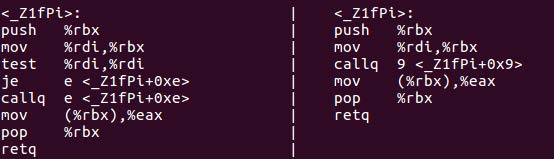
\includegraphics[width=0.9\textwidth]{content/3/chapter11/images/7.jpg}\\
圖11.7 - 為\texttt{f()}函數生成的x86彙編碼(左)和(右)沒有指針檢查
\end{center}

測試指令執行與null(零)的比較,後面跟著條件跳轉——這就是\texttt{if}語句在彙編中的樣子。 

為什麼編譯器沒有優化掉檢查呢?要回答這個問題,必須弄清楚在什麼條件下優化會改變程序的(良好定義的)行為。

要使優化無效,需要以下兩點:

\begin{itemize}
\item 
首先,\texttt{g()}函數必須知道指針\texttt{p}是否為空。這是可能的,例如:\texttt{p}也可以讓\texttt{f()}的調用者存儲在一個全局變量中。

\item 
其次,如果\texttt{p}為空,則不能執行\texttt{return}。這也是可能的:如果\texttt{p}為空,\texttt{g()}可能會拋出一個異常。
\end{itemize}

對於與UB密切相關的C++優化的最後一個例子,將看一些不同的東西。\texttt{const}關鍵字對優化的影響,這將說明為什麼編譯器不能成功的優化某些代碼。

\begin{lstlisting}[style=styleCXX]
bool f(int x) { return x + 1 > x; }
\end{lstlisting}

正如所看到的,優化編譯器將從這個函數中刪除所有代碼,並將其替換為\texttt{return true}。現在讓函數做更多的工作:

\begin{lstlisting}[style=styleCXX]
void g(int y);
bool f(int x) {
	int y = x + 1;
	g(y);
	return y > x;
}
\end{lstlisting}

當然,可能會有同樣的優化,代碼可以重寫如下:

\begin{lstlisting}[style=styleCXX]
void g(int y);
bool f(int x) {
	g(x + 1);
	return x + 1 > x;
}
\end{lstlisting}

必須調用\texttt{g()},但函數仍然返回true。在不陷入未定義行為的情況下,比較不會產生結果。同樣,大多數編譯器都會進行這種優化。以通過比較原始代碼生成的彙編碼,和完全手工優化的代碼生成的彙編碼來證實這一點:

\begin{lstlisting}[style=styleCXX]
void g(int y);
bool f(int x) {
	g(x + 1);
	return true;
}
\end{lstlisting}

可能進行優化的原因是\texttt{g()}函數不更改其參數。同一段代碼中,如果\texttt{g()}通過引用接收實參,則不再可能進行優化:

\begin{lstlisting}[style=styleCXX]
void g(int& y);
bool f(int x) {
	int y = x + 1;
	g(y);
	return y > x;
}
\end{lstlisting}

現在\texttt{g()}函數可以改變\texttt{y}的值,所以每次都要進行比較。如果函數\texttt{g()}的目的不是改變它的參數,就可以通過值進行傳遞。另一個選項是傳遞\texttt{const}引用,雖然對於小型類型(如整數)沒有理由這樣做,但模板代碼通常會生成這樣的函數。這個例子中,代碼看起來會是這樣:

\hspace*{\fill} \\ %插入空行
\noindent
\textbf{10\_const.C}
\begin{lstlisting}[style=styleCXX]
void g(const int& y);
bool f(int x) {
	int y = x + 1;
	g(y);
	return y > x;
}
\end{lstlisting}

對彙編程序的檢查表明\texttt{return}語句沒有進行優化,仍然進行比較。當然,編譯器不做某種優化證明瞭什麼,說明沒有優化器是完美的,但不做優化是有原因的。不管代碼怎麼樣,C++標準並不保證\texttt{g()}函數不改變它的參數!下面是一個完全符合標準的實現:

\begin{lstlisting}[style=styleCXX]
void g(const int& y) { ++const_cast<int&>(y); }
bool f(int x) {
	int y = x + 1;
	g(y);
	return y > x;
}
\end{lstlisting}

函數允許棄用\texttt{const}。結果定義的很好,並在標準中指定(這並不能使它成為好的代碼,只是有效的代碼)。但是,有一個例外:在創建時聲明為\texttt{const}的對象轉換為\texttt{const}。舉例來說,這是一個很好的定義(但不明智):

\begin{lstlisting}[style=styleCXX]
int x = 0;
const int& y = x;
const_cast<int&>(y) = 1;
\end{lstlisting}

這是會有UB的版本:

\begin{lstlisting}[style=styleCXX]
const int x = 0;
const int& y = x;
const_cast<int&>(y) = 1;
\end{lstlisting}

可以通過將中間變量\texttt{y}聲明為\texttt{const}來利用UB:

\begin{lstlisting}[style=styleCXX]
void g(const int& y);
bool f(int x) {
	const int y = x + 1;
	g(y);
	return y > x;
}
\end{lstlisting}

現在編譯器可以假設函數總是返回true。更改它的唯一方法是創造UB,而編譯器不需要UB。在寫這本書的時候,還不知道有編譯器會做這種優化。

考慮到這一點,在對使用\texttt{const}來進行優化,有什麼建議呢?

\begin{itemize}
\item 
如果值沒有改變,將它聲明為\texttt{const}。正確性很重要,但這確實可以支持一些優化,特別是當編譯器可以通過在編譯時計算表達式來傳播\texttt{const}時。

\item 
更好的優化方法是,若該值在編譯時已知,則將其聲明為\texttt{constexpr}。

\item 
通過\texttt{const}引用傳遞形參給函數沒有任何優化作用,因為編譯器必須假定函數可能會拋棄\texttt{const}(如果函數是內聯的,編譯器知道發生了什麼,但如何聲明形參就無關緊要了)。另一方面,這是將\texttt{const}對象傳遞給函數的唯一方法,因此,只要有可能,請將引用聲明為\texttt{const}(更重要的為了清晰的表明意圖)。

\item 
對於小類型,按值傳遞比按引用傳遞更有效(這不適用於內聯函數)。這很難與模板生成的泛型函數相協調(不要假設模板總是內聯的,大型模板函數通常不是)。有一些方法可以強制特定類型的值傳遞,但會使模板代碼更加繁瑣。不要一開始就寫這樣的代碼,只有當測試結果表明,對於特定的代碼段,這種工作是合理的時再這樣做。

\end{itemize}

我們已經詳細探討了C++中的UB如何影響C++代碼的優化。現在是時候回到正題,瞭解如何在自己的程序中利用UB了。
























